\documentclass{article}
\usepackage[utf8]{inputenc}
\usepackage[russian]{babel}
\usepackage{graphicx}

\title{homeWork#1}
\author{Kalinina Ksenia A-13a-19 }
\date{2022}

\begin{document}

\maketitle

\section
{Задание №1. Построить конечный автомат, распознающий язык}

1.1 \(L = \{w \in \{{a,b,c\} ^*|\ |w|_c=1\}}\)

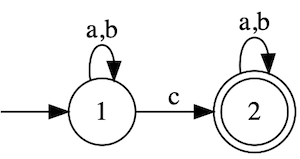
\includegraphics{graph_1_1}

1.2 \(L = \{w \in a,b^*| \ |w|_a\leq 2,\ |w|_b\geq 2\}}\)

\begin{tabular}{ | c | c | c | }
\hline
& a & b \\ \hline
q1,q4 & q2,q4 & q1,q5 \\ \hline
q1,q5 & q2,q5 & q1,q6 \\ \hline
q1,q6 & q2,q6 & q1,q6 \\ \hline
q2,q4 & q3,q4 & q2,q5 \\ \hline
q2,q5 & q3,q5 & q2,q6 \\ \hline
q2,q6 & q3,q6 & q2,q6 \\ \hline
q3,q4 & \emptyset & q3,q5 \\ \hline
q3,q5 & \emptyset & q3,q6 \\ \hline
q3,q6 & \emptyset & q3,q6 \\
\hline
\end{tabular}

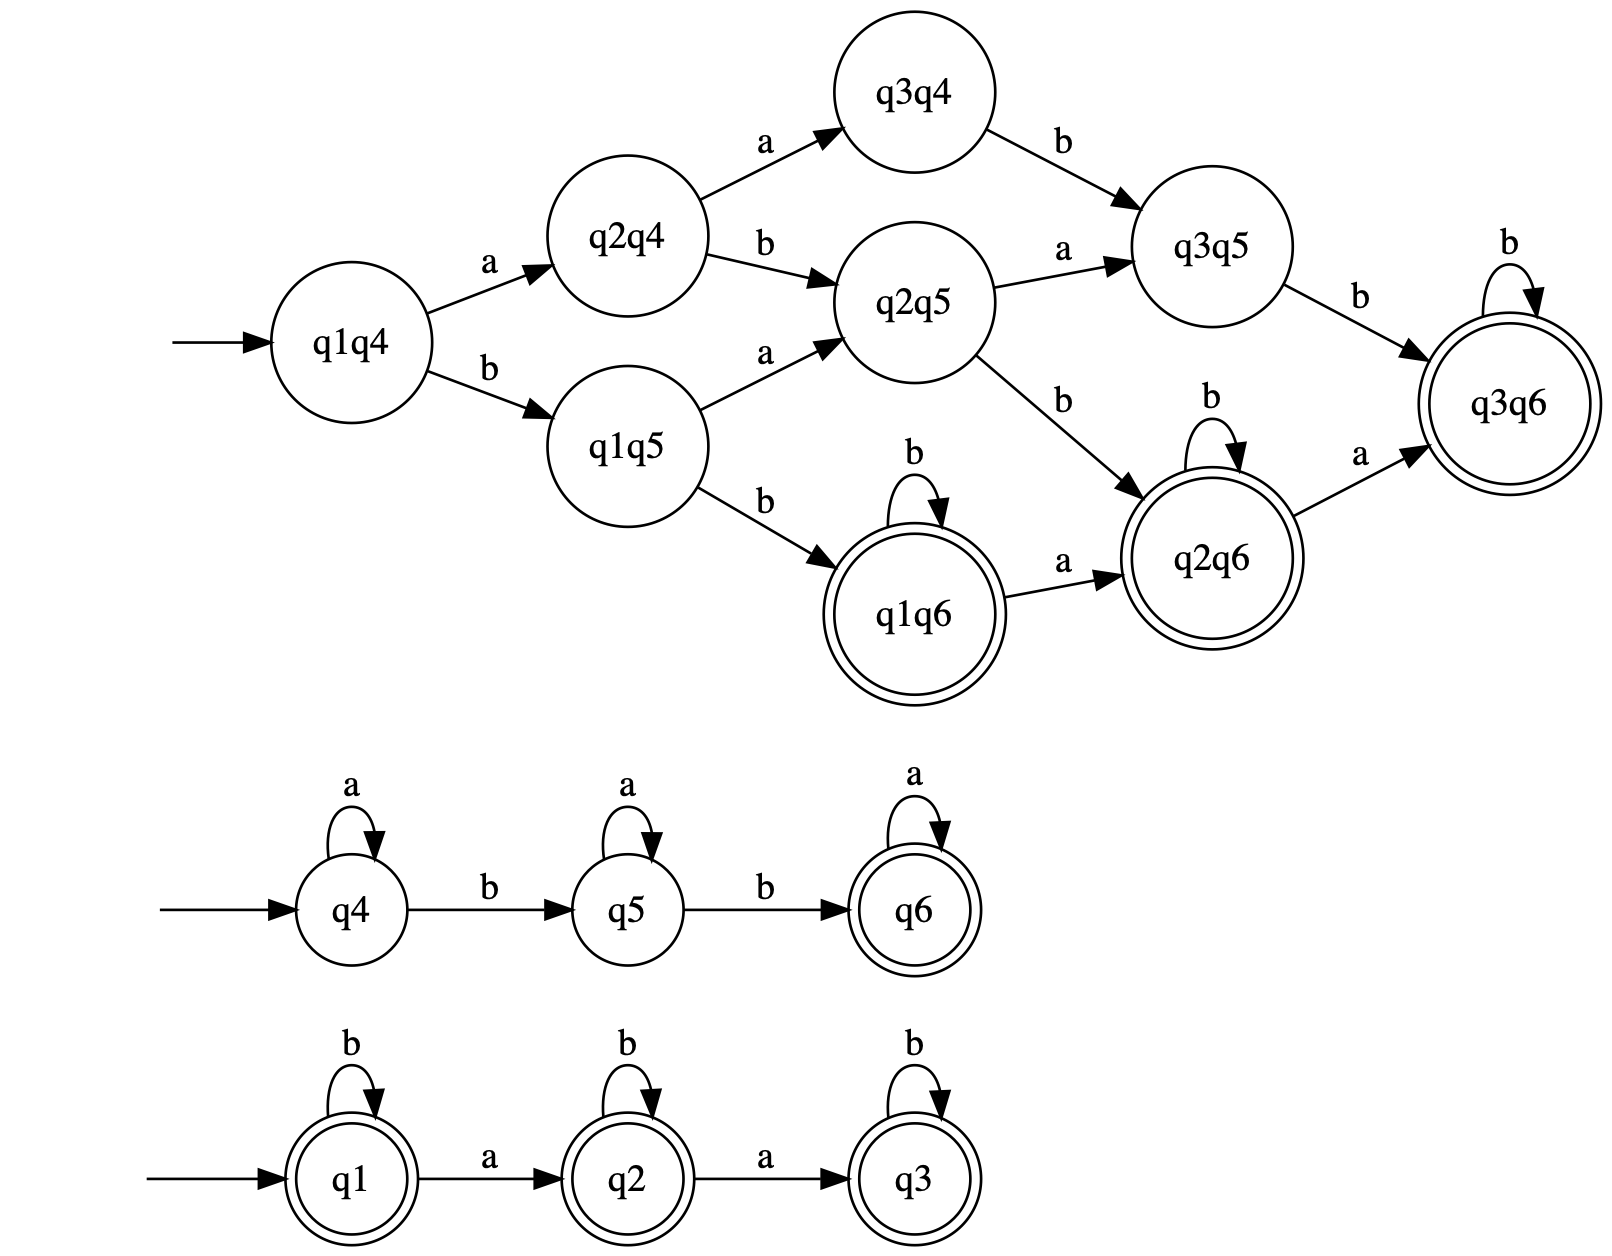
\includegraphics[width = 15cm, height = 15 cm]{1-2.png}

1.3 \(L = \{w \in \{{a,b\} ^*|\ |w|_a \neq |w|_b}\}^*\)
\newline
Невозможно описать с помощью ДКА, т.к. имеется необходимость запоминать число символов хотя бы одного (а или б)
\newpage

1.4 \(L = \{w \in a,b^*| \ ww = www}\}\)

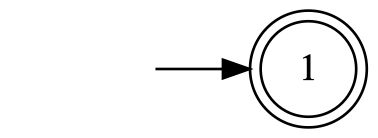
\includegraphics[width = 5cm, height =3 cm]{1-4.png}

\section
{Задание №2. Построить конечный автомат, используя прямое произведение}

2.1 \(L_1 = \{w \in \{a,b\} |\ |w|_a \geq 2 \land |w|_b \geq 2}\}\)

\begin{tabular}{ | c | c | c | }
\hline
& a & b \\ \hline
q1,q4 & q2,q4 & q1,q5 \\ \hline
q1,q5 & q2,q5 & q1,q6 \\ \hline
q1,q6 & q2,q6 & q1,q6 \\ \hline
q2,q4 & q3,q4 & q2,q5 \\ \hline
q2,q5 & q3,q5 & q2,q6 \\ \hline
q2,q6 & q3,q6 & q2,q6 \\ \hline
q3,q4 & q3,q4 & q3,q5 \\ \hline
q3,q5 & q3,q5 & q3,q6 \\ \hline
q3,q6 & q3,q6 & q3,q6 \\
\hline
\end{tabular}

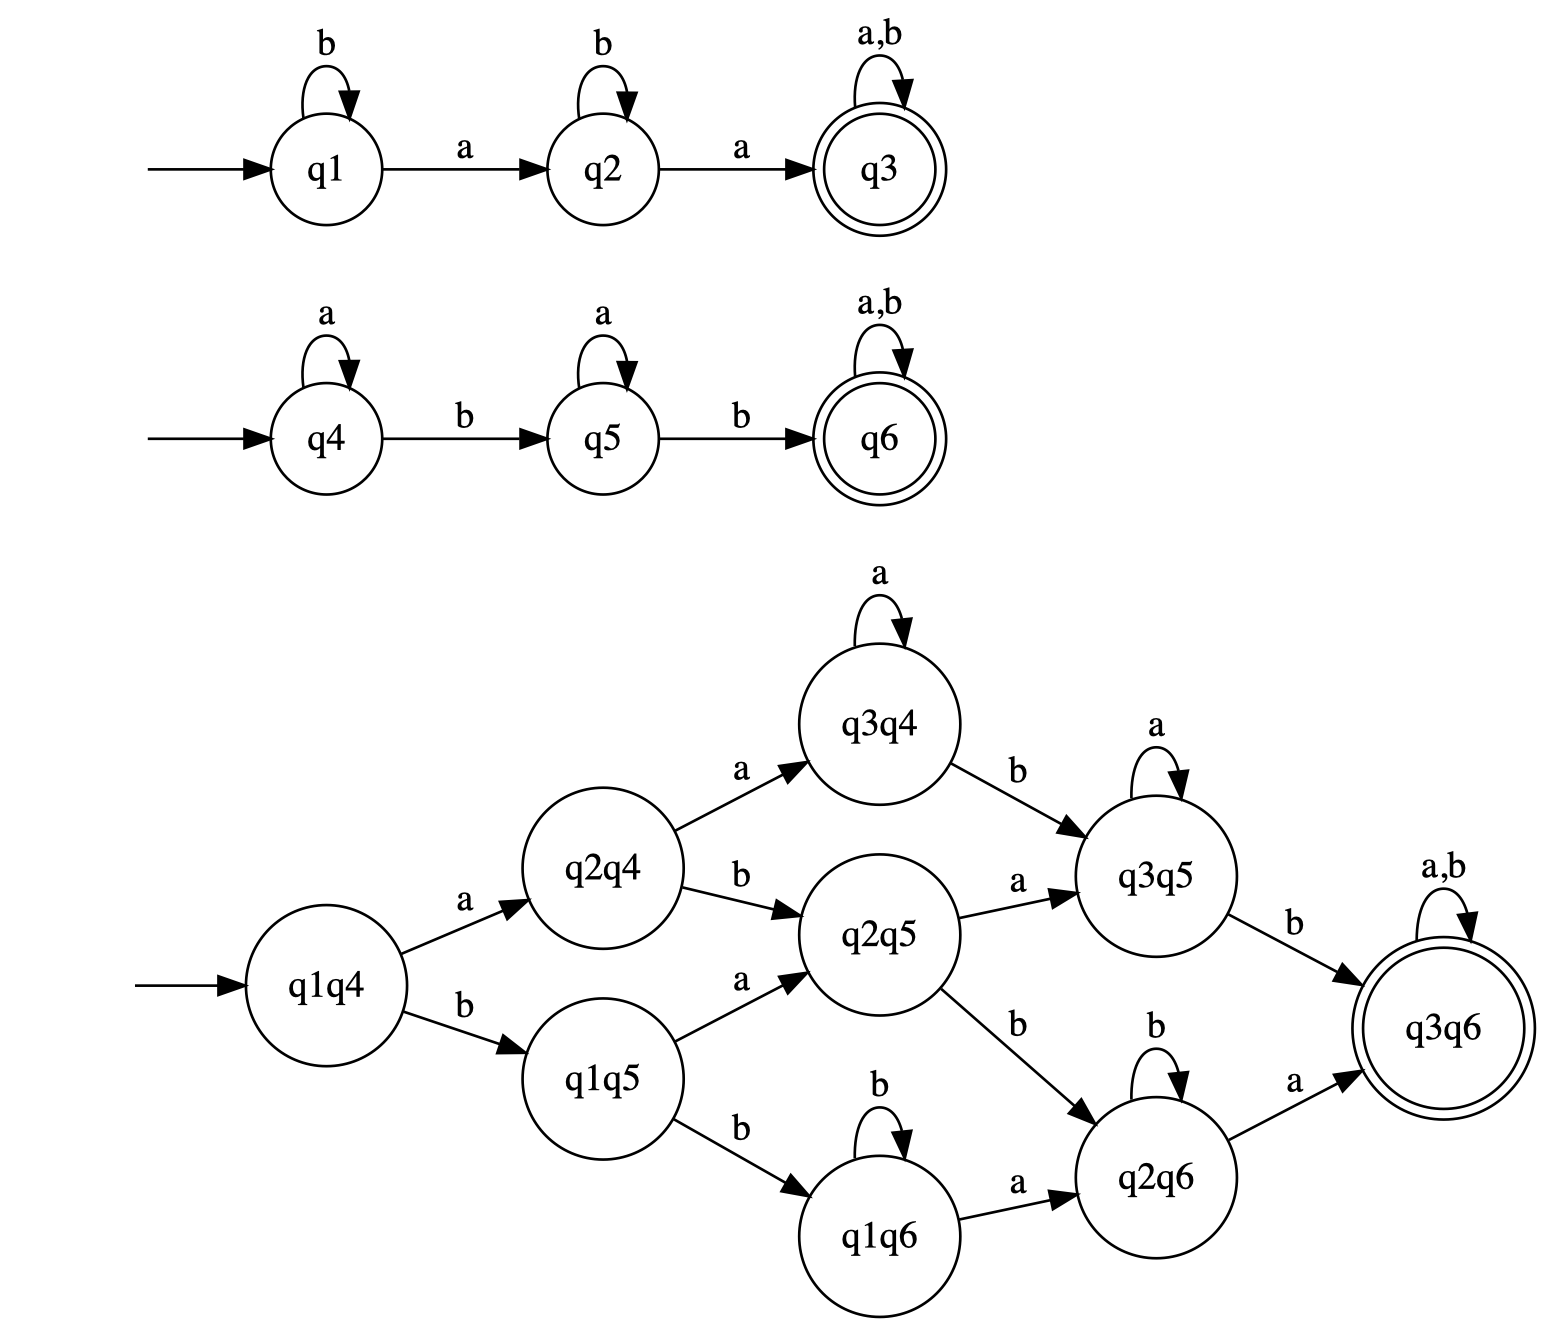
\includegraphics[width = 15cm, height = 10 cm]{2-1.png}
\newpage
2.2 \(L_2 = \{w \in \{a,b\}^* |\ |w| \geq 3 \land |w| \ mod 2 \neq 0\}\)

\begin{tabular}{ | c | c | c | }
\hline
& a & b \\ \hline
q1,q5 & q2,q6 & q2,q6 \\ \hline
q1,q6 & q2,q5 & q2,q5 \\ \hline
q2,q5 & q3,q6 & q3,q6 \\ \hline
q2,q6 & q3,q5 & q3,q5 \\ \hline
q3,q5 & q4,q6 & q4,q6 \\ \hline
q3,q6 & q4,q5 & q4,q5 \\ \hline
q4,q5 & q4,q6 & q4,q6 \\ \hline
q4,q6 & q4,q5 & q4,q5 \\ \hline
\end{tabular}

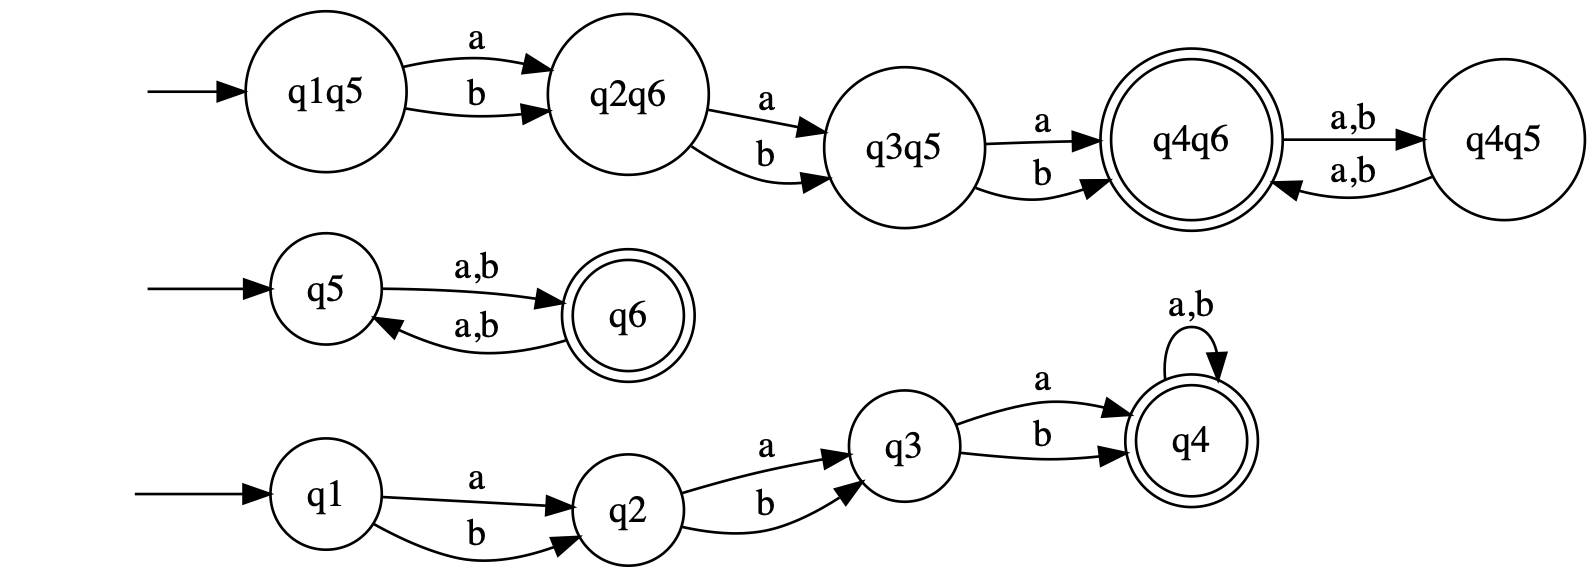
\includegraphics[width = 15cm, height = 10cm]{2-2.png}
\newpage

2.3 \(L_3 = \{w \in \{a,b\}^* |\ (|w|_a\ mod \ 2 = 0) \land (|w|_b \ mod \ 3 = 0)\}\)

\begin{tabular}{ | c | c | c | }
\hline
& a & b \\ \hline
q1,q4 & q1,q5 & q2,q4 \\ \hline
q1,q5 & q1,q4 & q2,q5 \\ \hline
q2,q4 & q2,q5 & q3,q4 \\ \hline
q2,q5 & q2,q4 & q3,q5 \\ \hline
q3,q4 & q3,q5 & q1,q4 \\ \hline
q3,q5 & q3,q4 & q1,q5 \\ \hline
\end{tabular}

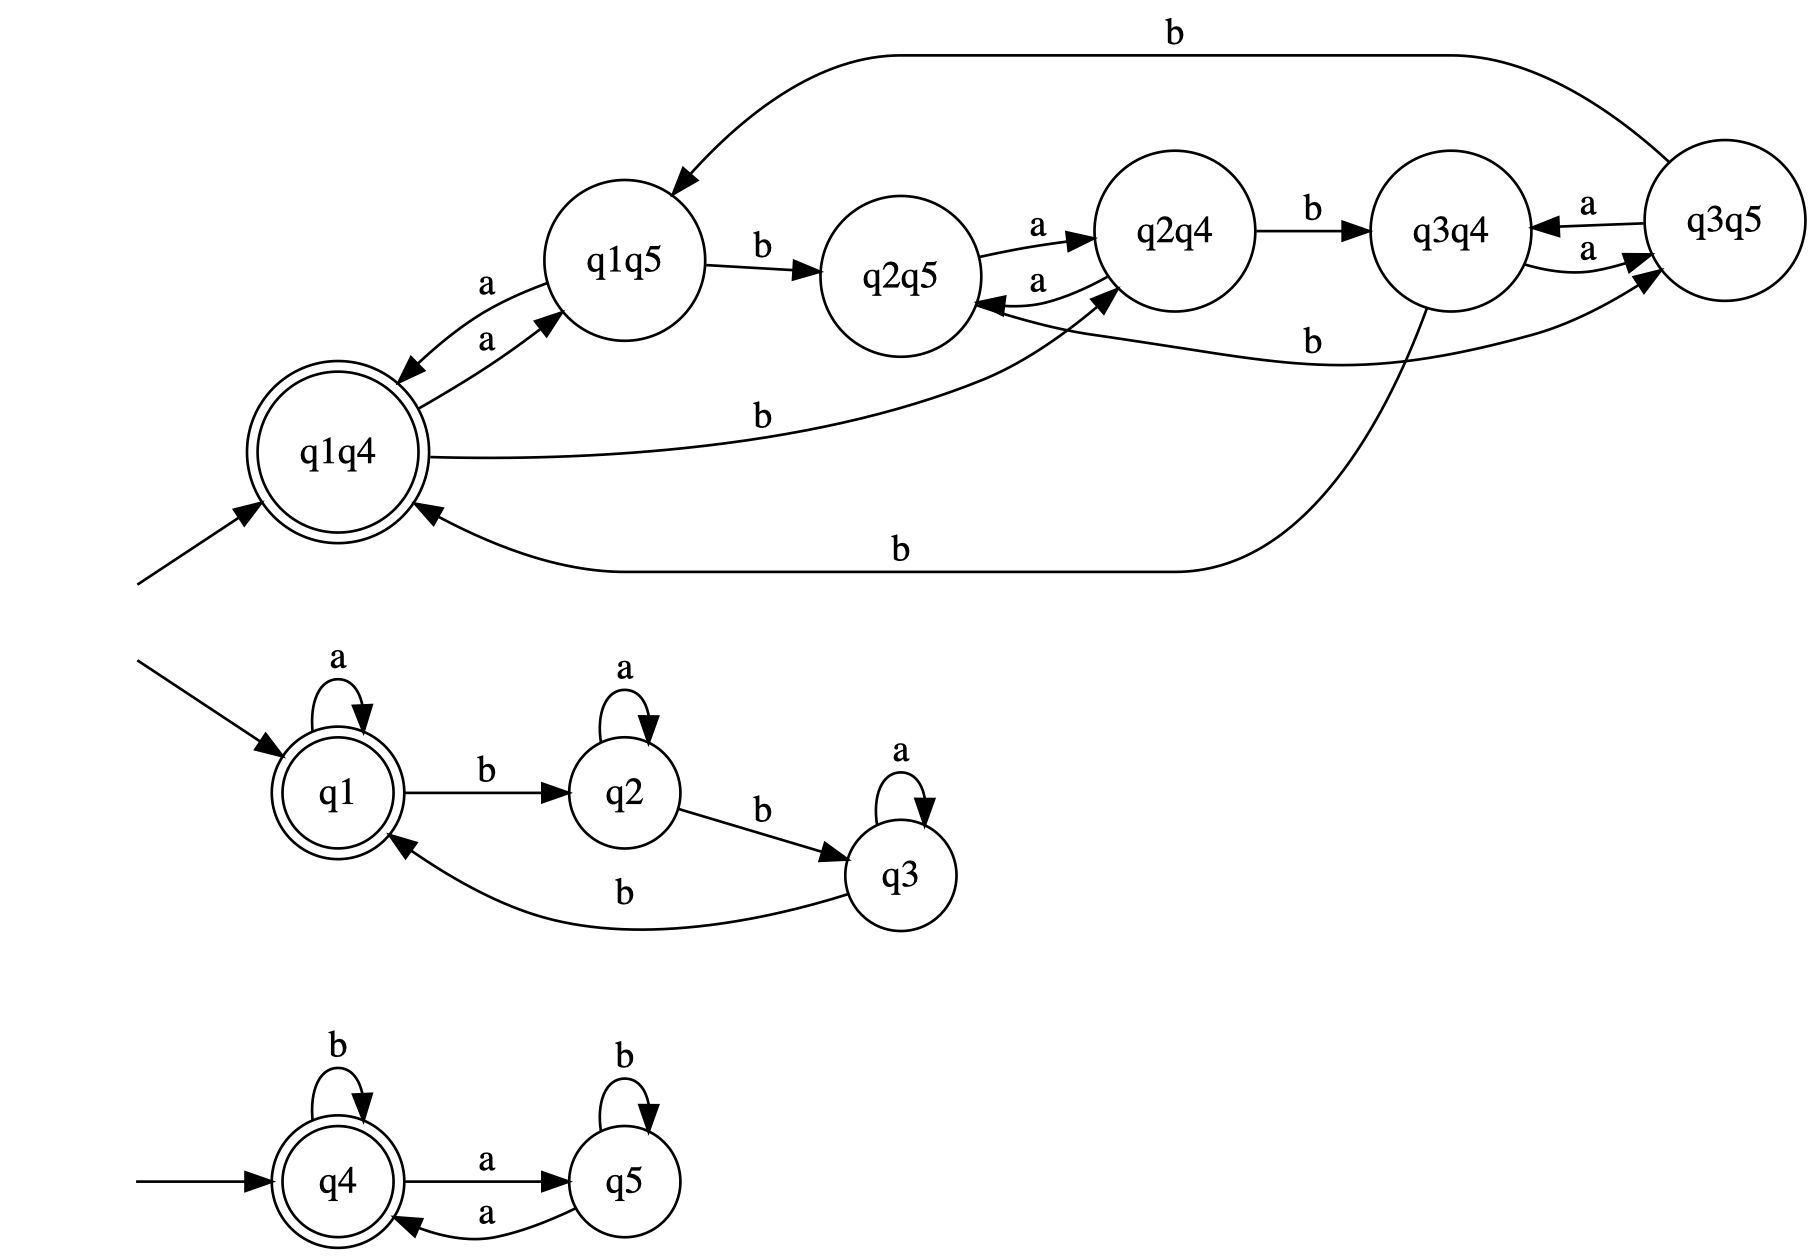
\includegraphics[width = 15cm, height = 10cm]{2-3.png}
\newpage

2.4 \(L_4 = \overline L_3 \)

T_4 = Q_3\ T_3 = q1q4,q1q5,q2q4,q2q5,q3q4,q3q5

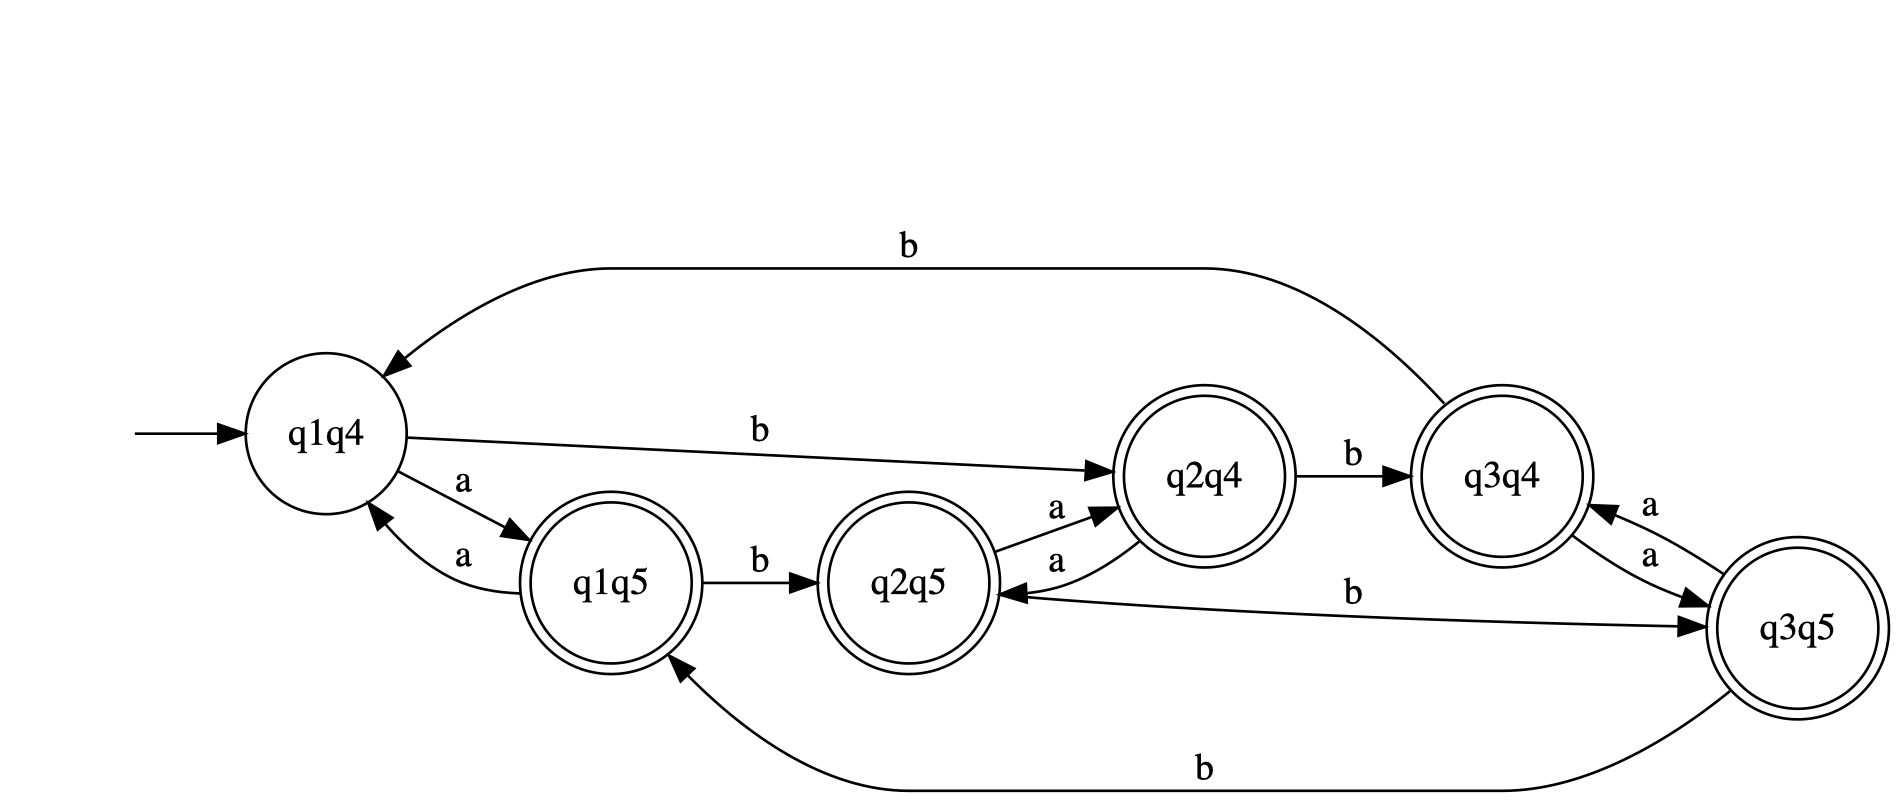
\includegraphics[width = 15cm, height = 8 cm]{2-4.png}

\newpage
\section
{Задание №3. Построить минимальный ДКА по регулярному выражению}

3.1 \((ab + aba)^* a \)
\newline
НКА

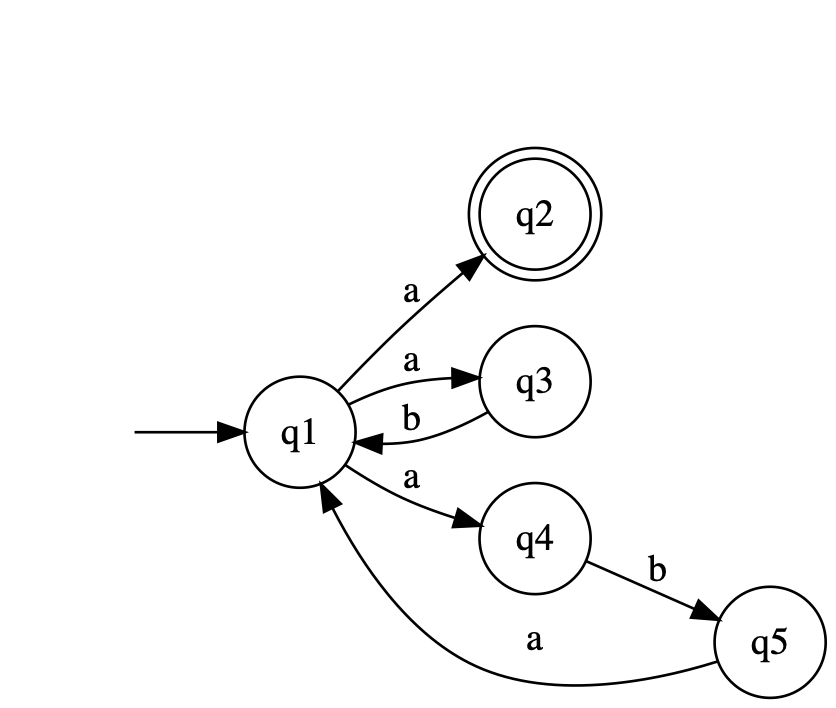
\includegraphics[width = 15cm, height = 8cm]{3-1_нка.png}

Строим по алгоритму Томпсона ДКА

\begin{tabular}{ | c | c | c | }
\hline
& a & b \\ \hline
q1 & q2,q3,q4 & \\ \hline
q2,q3,q4 & & q1,q5 \\ \hline
q1,q5 & q1,q2,q3,q4 & \\ \hline
q1,q2,q3,q4 & q2,q3,q4 & q1,q5 \\
\hline
\end{tabular}

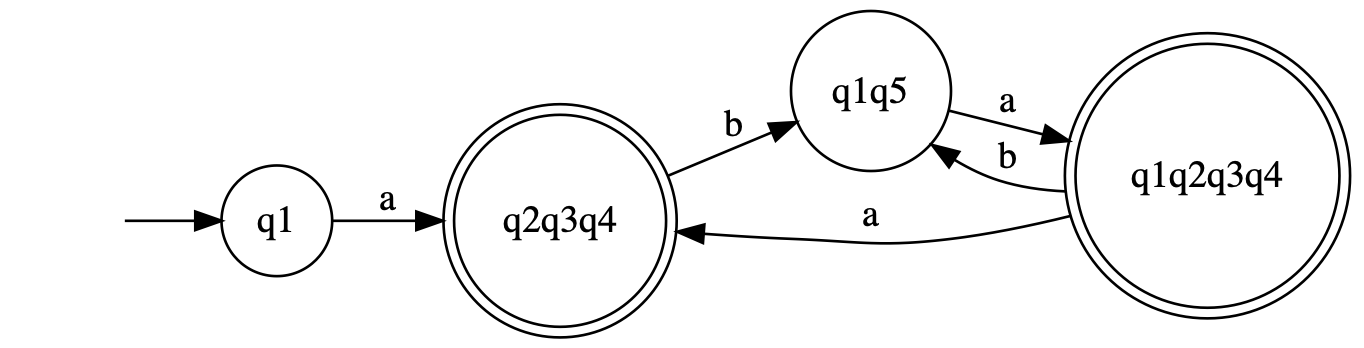
\includegraphics[width = 15cm, height = 5cm]{3-1дка.png}

\newpage

3.2 \((a(a(ab)^*b)^*(ab)^* \)
\newline
НКА

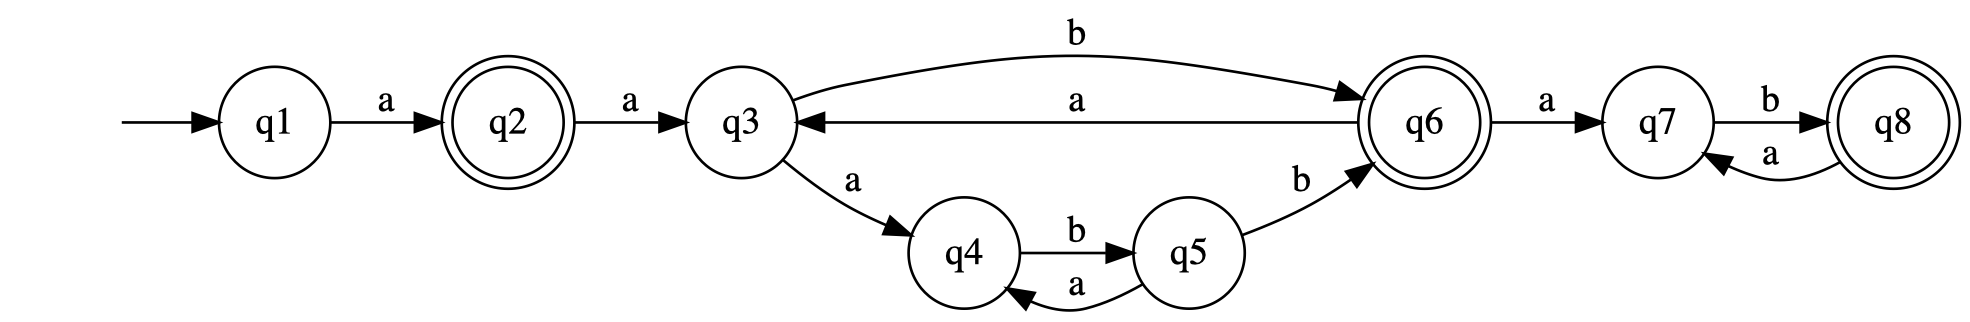
\includegraphics[width = 15cm, height = 5cm]{3-2_нка.png}

Строим по алгоритму Томпсона ДКА:

\begin{tabular}{ | c | c | c | }
\hline
& a & b \\ \hline
q1 & q2,q3,q4 & \\ \hline
q2,q3,q4 & & q1,q5 \\ \hline
q1,q5 & q1,q2,q3,q4 & \\ \hline
q1,q2,q3,q4 & q2,q3,q4 & q1,q5 \\ \hline
\end{tabular}

\newline

ДКА

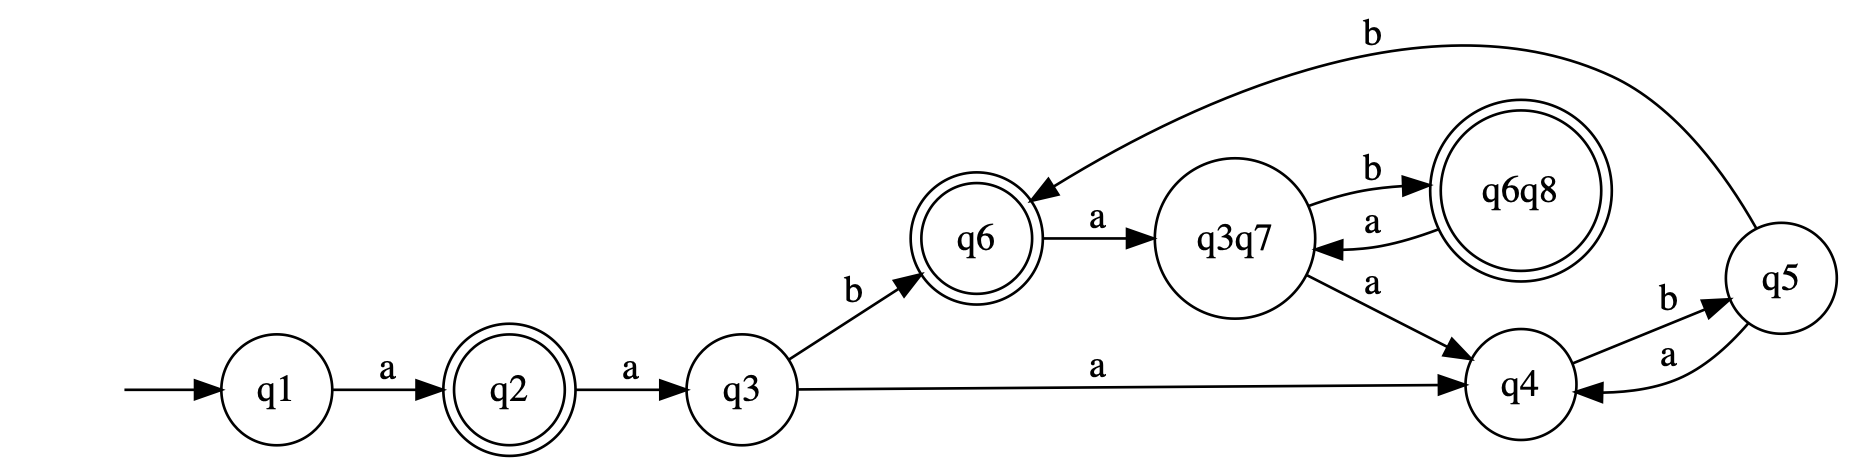
\includegraphics[width = 15cm, height = 5cm]{3-2_дка.png}

\begin{tabular}{ | c | c | c | c | c | c | c | c | c | }
\hline
& q1 & q2 & q3 & q4 & q5 & q6 & q3q7 & q6q8 \\ \hline
q1 & & + & + & + & + & + & + & + \\ \hline
q2 & + & & + & + & + & + & + & + \\ \hline
q3 & + & + & & + & + & + & & + \\ \hline
q4 & + & + & + & & + & + & + & + \\ \hline
q5 & + & + & + & + & & + & + & + \\ \hline
q6 & + & + & + & + & + & & + & \\ \hline
q3,q7 & + & + & & + & + & + & & + \\ \hline
q6,q8 & + & + & + & + & + & & + & \\ \hline
\end{tabular}

\newpage

ДКА-2

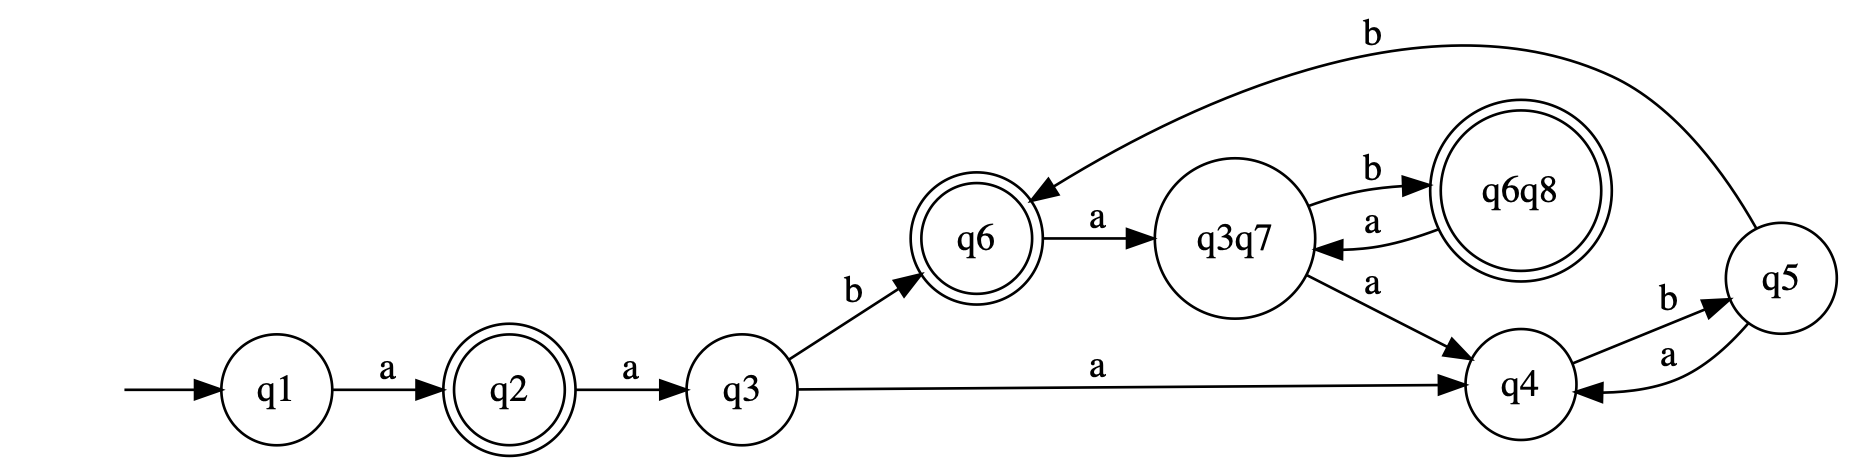
\includegraphics[width = 15cm, height = 5cm]{3-2_дка_версия2.png}

\newpage

3.3 \((a + (a + b)(a + b)b)^*\)
\newline
НКА
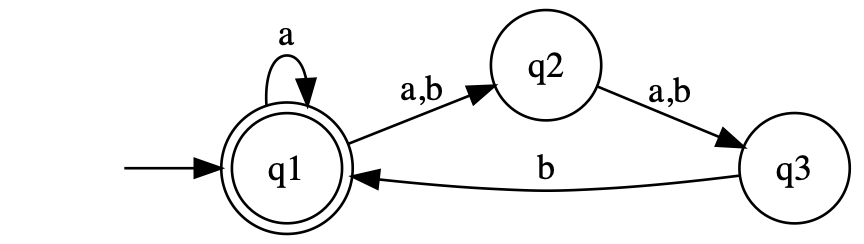
\includegraphics[width = 10cm, height = 5cm]{3-3нка.png}

Строим по алгоритму Томпсона ДКА:

\begin{tabular}{ | c | c | c | }
\hline
& a & b \\ \hline
q1 & q1,q2 & q2 \\ \hline
q2 & q3 & q3 \\ \hline
q3 & & q6 \\ \hline
q1,q2 & q1,q2,q3 & q2,q3 \\ \hline
q2,q3 & q1,q3 & q3 \\ \hline
q1,q3,q4 & q1,q2 & q1,q2 \\ \hline
q1,q2,q3 & q1,q2,q3 & q1,q2,q3 \\ \hline
\end{tabular}

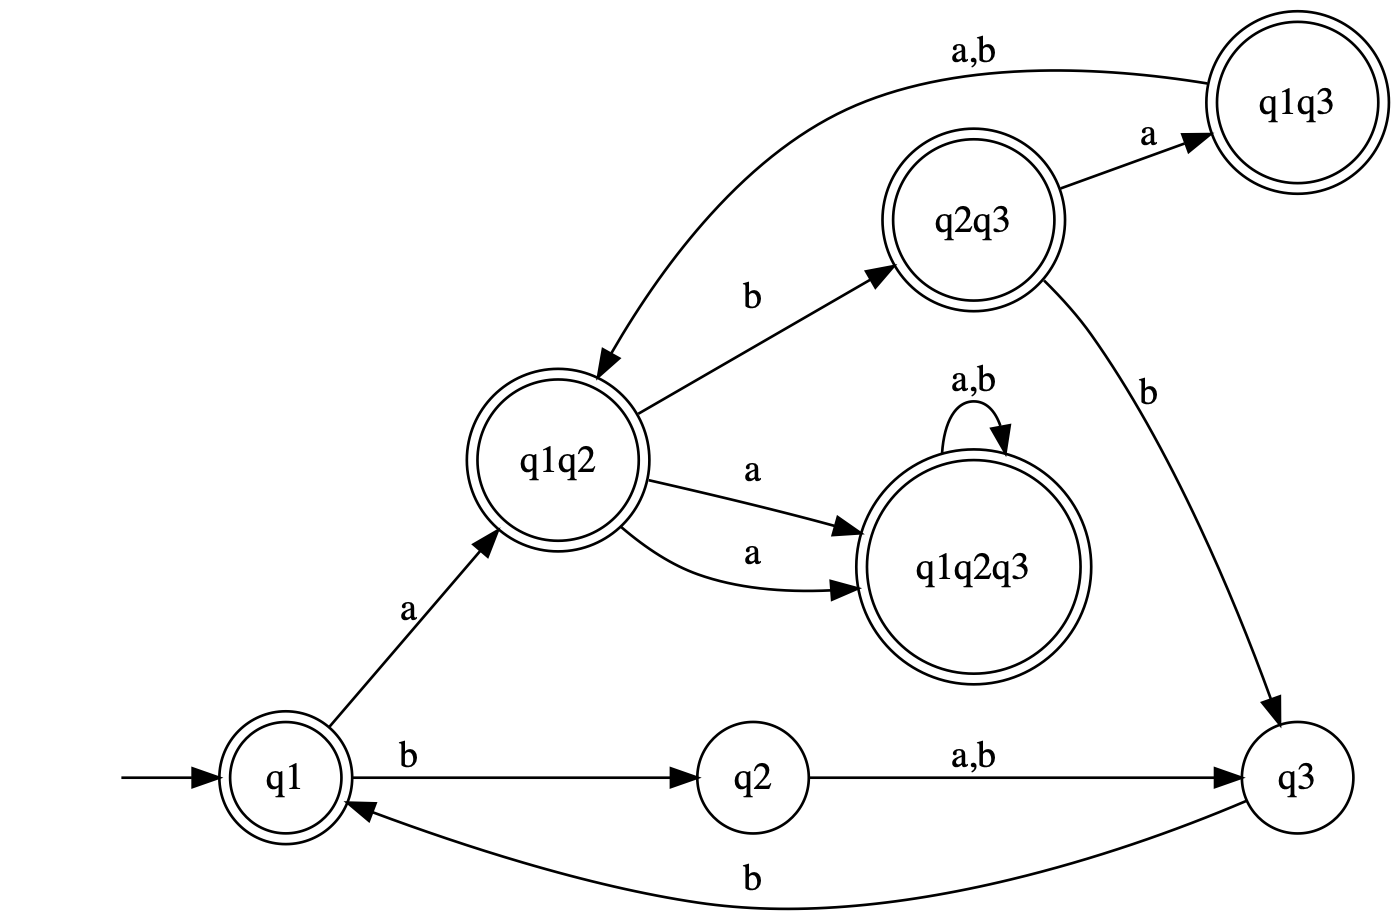
\includegraphics[width = 15cm, height = 8cm]{3-3дка.png}

\newpage

3.4 \((b + c)((ab)^*c + (ba)^*)^*\)

\newline

НКА

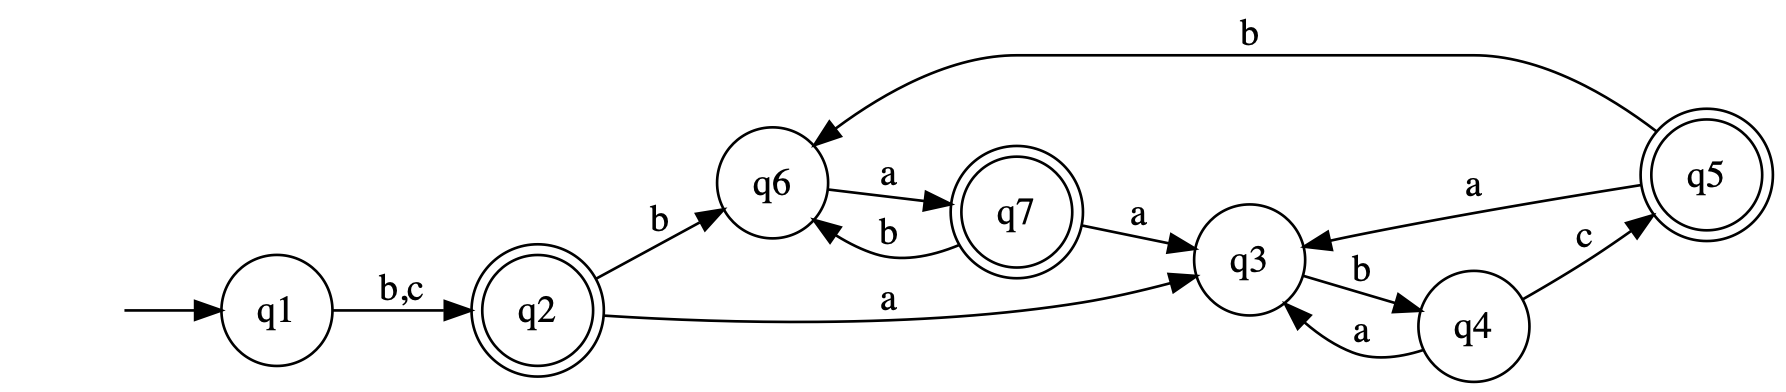
\includegraphics[width = 15cm, height = 5cm]{3-4нка.png}

Строим по алгоритму Томпсона ДКА:

\begin{tabular}{ | c | c | c | c | }
\hline
& a & b & c \\ \hline
q1 & & q2 & q2 \\ \hline
q2 & q3 & q6 & \\ \hline
q3 & & q4 & \\ \hline
q4 & q3 & & q5\\ \hline
q5 & q3 & q6 & \\ \hline
q6 & q7 & & \\ \hline
q7 & q3 & q6 & \\ \hline
\end{tabular}

\begin{tabular}{ | c | c | c | c | c | c | c | c | }
\hline
& q1 & q2 & q3 & q4 & q5 & q6 & q7 \\ \hline
q1 & & + & + & + & + & + & + \\ \hline
q2 & + & & + & + & & + & \\ \hline
q3 & + & + & & + & + & + & + \\ \hline
q4 & + & + & + & & + & + & + \\ \hline
q5 & + & & + & + & & + & \\ \hline
q6 & + & + & + & + & + & & + \\ \hline
q7 & + & & + & + & & + & \\ \hline
\end{tabular}

ДКА

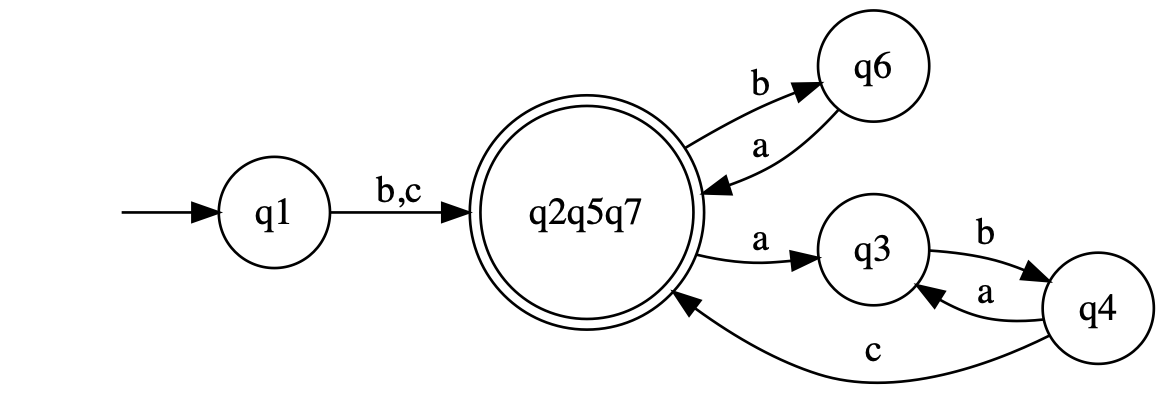
\includegraphics[width = 15cm, height = 5cm]{3-4дка.png}

\newpage

3.5 \((a + b)^+(aa + bb + abab + baba)(a + b)^+\)

НКА

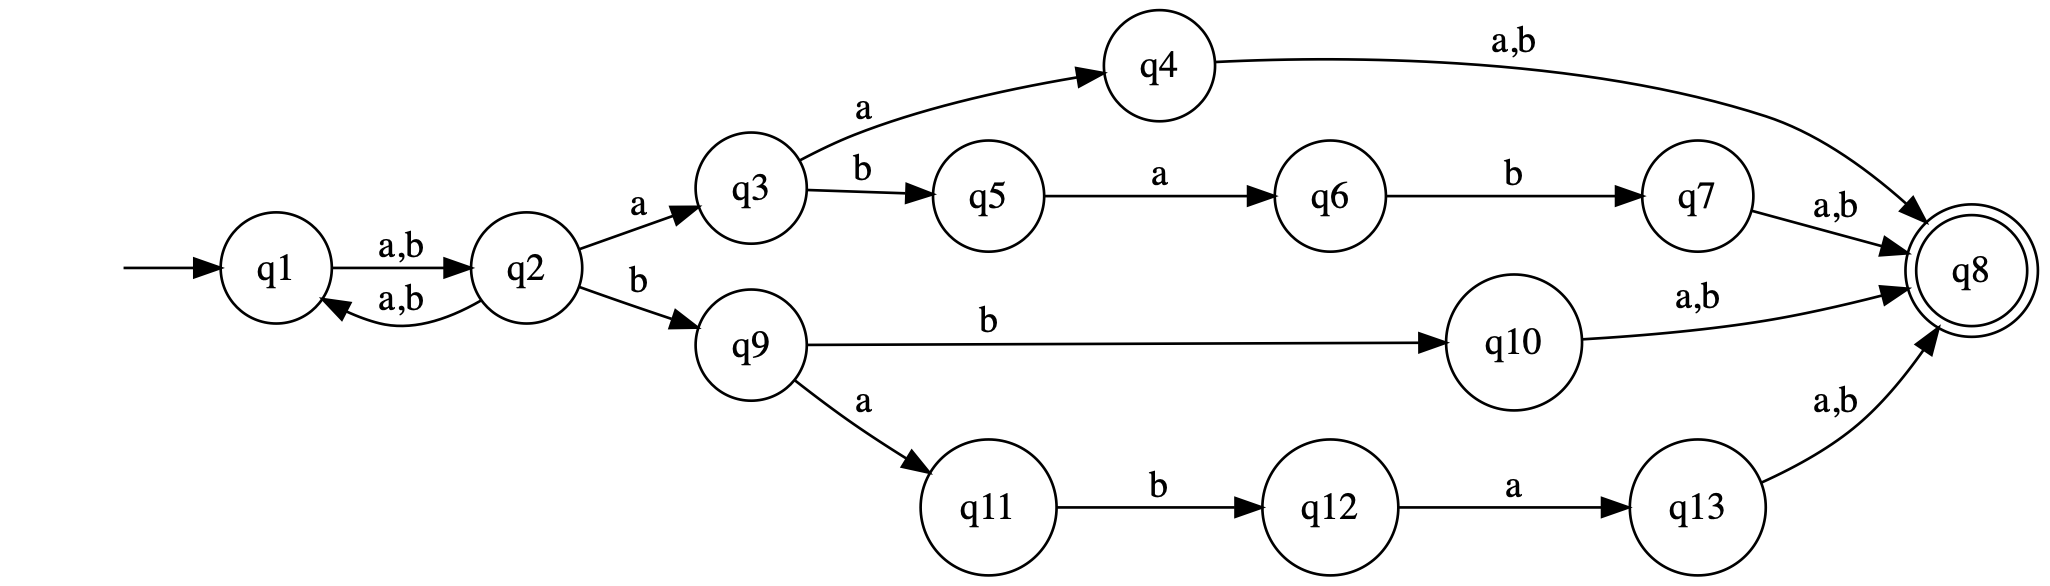
\includegraphics[width = 15cm, height = 8cm]{3-5нка.png}

\newpage
\section
{Задание №4. Определить является язык регулярным или нет}

4.1 \(L = \{(aab)^nb(aba)^m \ |\ n \geq 0, m \geq 0\}\)
Построить ДКА не удалось, значит язык регулярный.

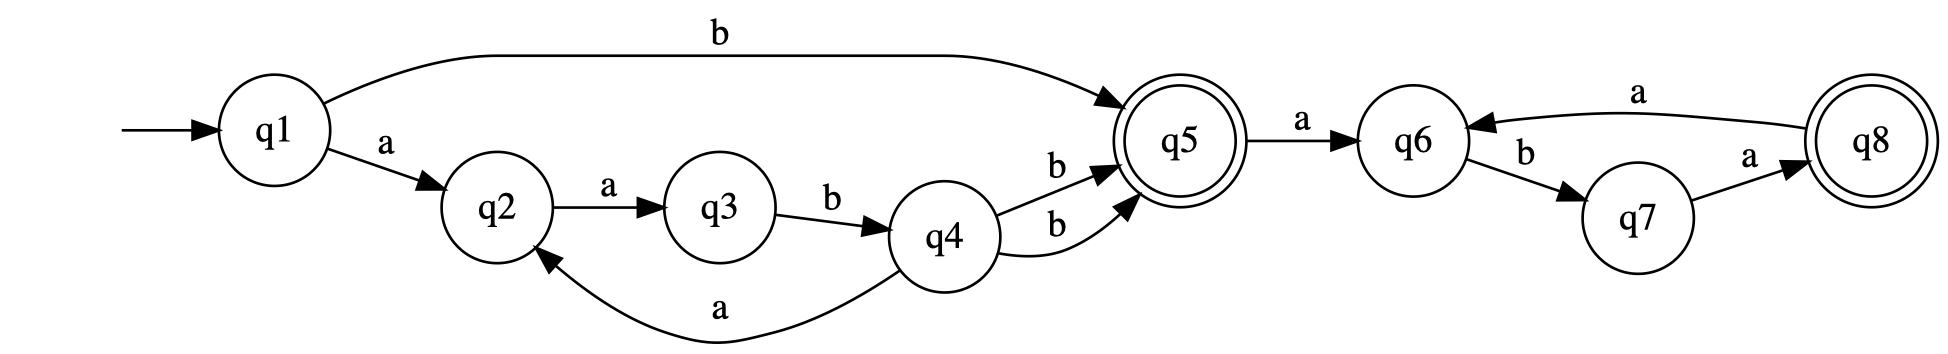
\includegraphics[width = 15cm, height = 3 cm]{4-1.png}

4.2 \(L = \{uaav | u \in \{a, b\}^*, \ v \in a, b^*, \ |u|_b \geq |v|_a\}\)

Рассмотрим слово: \(w = b^n aaa^n\) для любого n принадлежащего множеству натуральных чисел. Разобьем слово w на xyz так, что \(|xy| \leq n, |y|\neq 0\).
Тогда \(x = b^i, y = b^j, z=b^{n-i-j} aaa^n\), где \(i+j\) не больше n и j больше нуля.
Тогда \(xy^0z=a^ia^{n-i-j} b^n=a^{n-j}b^n \notin L \Rightarrow\) L не регулярный язык.
\newline

4.3 \(L = \{a^mw | w \in \{a, b\}^*, 1 \leq |w|_b \leq m\}\)

Рассмотрим слово: \(w = b^n a^n\) для любого n принадлежащего множеству натуральных чисел, тогда \(|w| = n + n \geq n\). Разобьем слово w на xyz так, что \(|xy| \leq n, |y|\neq 0\).
x = a^i y=a^j z=a^{n-i-j}b^n, где \(i+j\) не больше n и j больше нуля. 
Тогда \(xy^0z=a^ia^{n-i-j}b^n=a^{n-j}b^n \notin L \Rightarrow\) L не регулярный язык.
\newline

4.4 \(L = \{a^kb^ma^n \ | \ k = n \vee m \ge 0\}\)

Рассмотрим слово \(w = a^n b a^n\) для любого n принадлежащего множеству натуральных чисел, тогда |w| = n+1+n \gt n. Разобьем слово w на xyz так, что \(|xy| \leq n,
|y|\neq 0\).
x = a^i y=a^j z=a^{n-i-j}ba^n, где \(i+j\) не больше n, и j больше нуля. 
Тогда \(xy^2z=a^ia^{2j}a^{n-i-j}ba^n=a^{n+j}ba^n \notin L \Rightarrow\) L не регулярный язык.
\newline

4.5 \(L = \{ucv | u \in \{a, b\}^*, v \in \{a, b\}^*, u \neq v^R\}\)

Рассмотрим слово \(w = (ab)^nc(ab)^n = \alpha_1\alpha_2...\alpha_{4n+1} \) для любого n принадлежащего множеству натуральных чисел, тогда \(|w| = 4n+1 \gt n\). Разобьем слово w на xyz так, что \(|xy| \leq n, |y|\neq 0\).
x=\alpha_1\alpha_2...\alpha_i , y= \alpha_{i+1}\alpha_{i+2}...\alpha_{i+j}, z=\alpha_{i+j+1}\alpha_{i+j+1}...\alpha_{4n+1}c(ab)^n, где \(i+j\) не больше n, и j больше нуля.
Тогда \(xy^2z=(\alpha_1\alpha_2...\alpha_i)(\alpha_{i+1}\alpha_{i+2}...\alpha_{i+j})^2(\alpha_{i+j+1}\alpha_{i+j+1}...\alpha_{4n+1}c(ab)^n) \notin L \Rightarrow\) L не регулярный язык.
\newline


\end{document}
